\documentclass[12pt, letterpaper, twoside, titlepage]{article}
% font size could be 10pt (default), 11pt or 12 pt
% paper size coulde be letterpaper (default), legalpaper, executivepaper,
% a4paper, a5paper or b5paper
% side coulde be oneside (default) or twoside 
% columns coulde be onecolumn (default) or twocolumn
% graphics coulde be final (default) or draft 
%
% titlepage coulde be notitlepage (default) or titlepage which 
% makes an extra page for title 
% 
% paper alignment coulde be portrait (default) or landscape 
%
% equations coulde be 
%   default number of the equation on the rigth and equation centered 
%   leqno number on the left and equation centered 
%   fleqn number on the rigth and  equation on the left side
%	

\usepackage{graphicx}
\usepackage{float}

\title{Understanding Chetco Calibration Tables}
\author{Alan Booker
	 
	}

\date{\today} 
% \date{\today} date coulde be today 
% \date{25.12.00} or be a certain date
% \date{ } or there is no date 
\begin{document}
% Hint: \title{what ever}, \author{who care} and \date{when ever} could stand 
% before or after the \begin{document} command 
% BUT the \maketitle command MUST come AFTER the \begin{document} command! 
\maketitle


\begin{abstract}
The Chetco SeaGuage G2 is designed to interface with sensors measuring quantities such as pressure, temperature, levels, etc. and convert them into virtual gauges displayable in vDash and/or NMEA PNG records to be displayed by listeners on an NMEA 2000 network. A complete description of all of the possible ways the device can be used is beyond the scope of this note. Focus will be on the 12 analog channels and the ways input signal conditioning and calibration tables can be used to implement a wide variety of sensor types
\end{abstract}

%\tableofcontents % create a table of contens 



\section{Calibration Tables}
Calibration Tables are designed to be easily loaded into the G2 in a compact form, making them a little bit cryptic for human consumption. Fortunately, it is rare to have to generate a table completely manually. That said, It is important to understand what is in a Calibration Table and how the values are used.  Here is a somewhat contrived partial table to show the individual parts.  A complete table would consist of the header and 256 rows of data.

\begin{figure}[hbt!]
  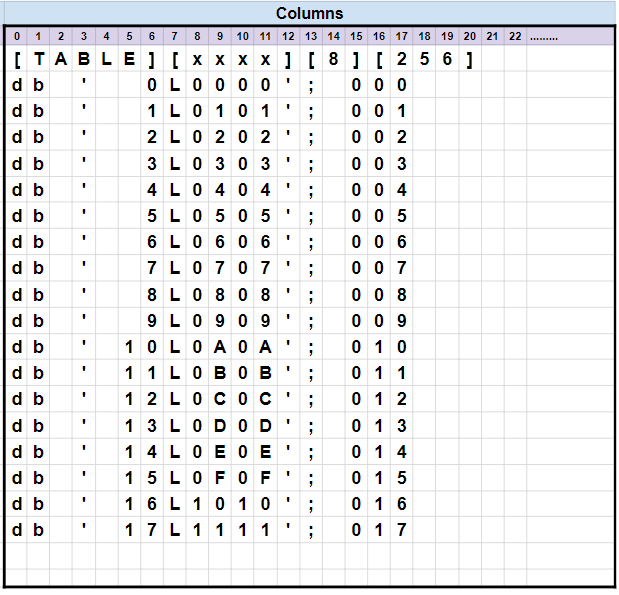
\includegraphics[width=\linewidth]{CaltableFigure2.png}
  \centering
  \caption{Partial Calibration Table}
  \label{fig:Cal_table}
\end{figure}

%Figure \ref{fig:Cal_table} shows a portion of a Calbrantion Table

The calibration table must conform to a strict format to be accepted by the G2. The first row begins with the identifier [TABLE] followed by 4 HEX characters of Table Address [xxxx]  Calibration Tables start at hex address [0800] and are 0x800 (2048) bytes long.  Refer to the table below for the correct address..

\begin{figure}[hbt!]
  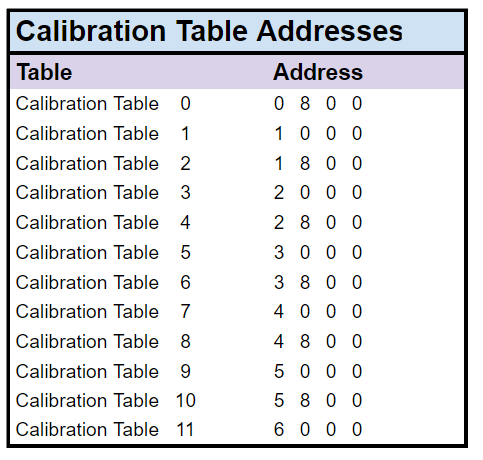
\includegraphics[ scale=0.4]{CalAddress.png}
  \centering
  \caption{ Calibration Table Address}
  \label{fig:Cal_Address}
\end{figure}

%Figure \ref{fig:Cal_Address} shows the mapping between the Calibration Table and address field

If vDash is used to load the Calibration Table, it will insert the correct value into the address based on which slot the table is configured. To finish out the header line, [8][256] indicates the table is 8 bytes per row and 256 data rows, respectively.  These values are fixed for a Calibration Table and should not be altered. Individual row descriptions are:

\begin{itemize}
\item Column 0-3 must be “db ‘” to indicate start of data field
\item Column 4-7 is the 4 character display value associated with the table index
\item Column 8-9 is two characters (HEX) used for NMEA 2000 lookup
\item Column 10-11 is two characters (HEX) used for graphic display lookup
\item Column 12-13 must be “’;” to indicate end of the data for that row
\item Column 14 – is a comment and usually starts with the table row index number for reference
\end{itemize}

\par
A correctly formed Calibration table is exactly 257 lines long (the [TABLE] \dots line + 256 lines of data)  In the course of this application note, several calibration tables will be developed. How the values are used by the G2 will be explained in the context of the examples. 

\section{Analog Inputs}
The G2 supports 12 inputs, numbered from 0 to 11.  A G2 can be ordered from the factory with Inputs 10 \& 11 configured  to electrically interface directly with K type thermocouples.   This document will assume that this configuration option was not selected and inputs 10 \& 11 are used as general analog inputs. It is also possible in vDash to configure which Analog Input corresponds to which Calibration table.  For example, physical Analog input 6 could be assigned to Calibration table 9.  While this does not affect the subsequent discussion, it is something to remember as the system is configured.  This diagram shows the major functional blocks and flow of an analog input channel.

\begin{figure}[hbt!]
  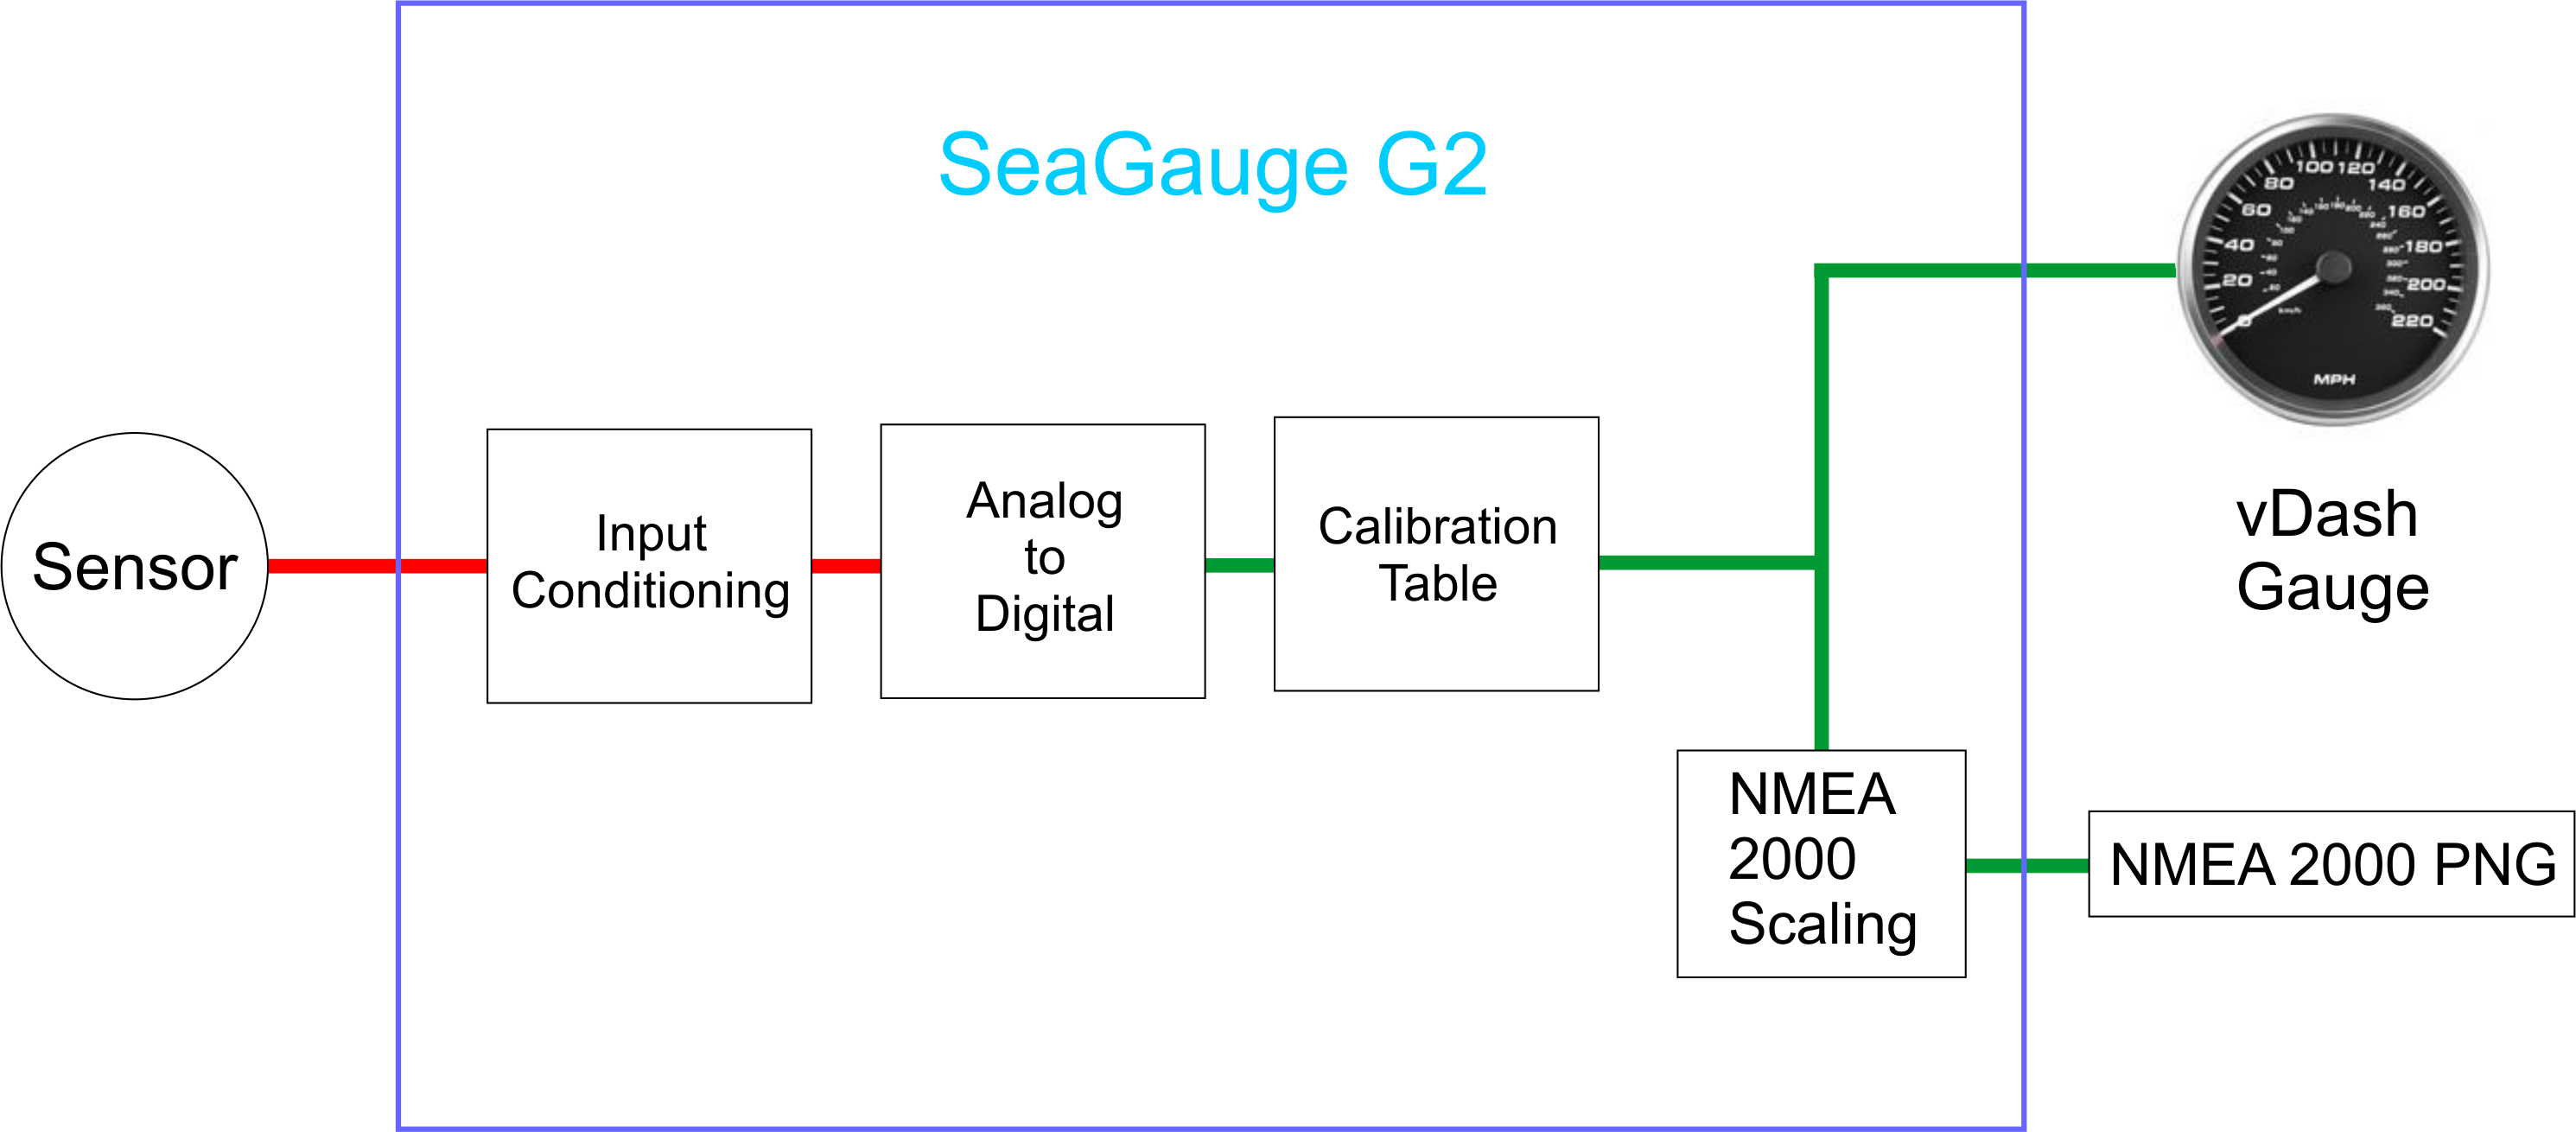
\includegraphics[width=\linewidth]{Sensor Example.png}
  \centering
  \caption{Analog Input Channel}
  \label{fig:Analog_Input}
\end{figure}

%Figure \ref{fig:Analog_Input} shows an Analog Input

\subsection{Sensor}
For purposes of this discussion, a sensor is a device that converts some physical quantity, like pressure, temperature, fluid level, etc. into a voltage (or a resistance).  There are many, many types of sensors that can be attached to a G2 with different ways of achieving this goal. While a complete discussion is beyond the scope of this note a couple of basic types will be covered 

\subsection{Input Conditioning}
Sensors come in many types and electrical interfaces.  To make it easier to attach to a G2 with minimal external components, the G2 provides several internal mechanisms designed to work with common commercial sensors. An example is voltage scaling, where the voltage swing of a sensor may be greater than a direct connection to the Analog to Digital convertor would support.  The direct connection to the Analog to Digital converter has a maximum limit of 2.5V.  For exampe, battery voltage monitoring would require something closer to a maximum of 15 Volts. Different Analog Inputs have different conditioning options, some of which are configurable with switches on the unit and/or factory customization.  A more indepth view into the specifics of available input conditioning will be addressed later (See  Section \ref{Input Conditioning} "Input Conditioning" on page \pageref{Input Conditioning})

\subsection{Analog to Digital}
 Simply, the Analog to Digital block converts an input voltage to a number.  A voltage from 0 - 2.5V is converted to a number in a linear range from 0 - 255. For example, 1.0 V yields a number of 102.  Each unit is $ 2.5 / 256$  volts, or a little under 10 mV per unit. 


\subsection{Calibration Table}
Even with input conditioning, available sensors rarely map neatly into 0 - 2.5V.  Some sensors do not have a linear relationship between the quantity being measured and the voltage produced.  Others may produce a baseline voltage when the physical quantity being measured is 0 to help distinguish between a 0 reading and a broken sensor. Calibration Tables can address these situations and more.  Recall that there are 256 data rows in a Calibration Table. The number from the Analog to Digital block is used to look up a data row, starting with the first row accessed when the voltage is 0.  This can be calculated b y$  Row\_Index = V_{input} * (256 / 2.5) $  This should be rounded down to the nearest integer.   To use 1.0 V as an example,  $ Row\_Index = 1.0 * (256 / 2.5) $ or 102.  Data table rows are numbered starting from 0; the first data table entry is row index 0.  The ability to provide custom data to the remainder of the G2 processing is powerful

\subsection{NMEA 2000 Scaling}
NMEA 2000 PGN fields use a wide variety of units and scaling internally.  For example, the Engine Temperature field found in PGN 127489  Engine Parameters Dynamic  is represented internally in units of 0.01 degrees Kelvin.  To permit a single Analog Input and corresponding Calibration Table to provide data for a gauge defined in an environment such as vDash and NMEA 2000 data, the G2 provides additional fixed scaling tailored for each field of each supported PGN.  An example of this will be shown later.

\subsection{vDash Style Gauge}
vDash style gauge configurations include items like color, type, position, label, etc.  The configuration option important for configuring Calibration Tables is range of the data. For example, 0 - 80 psi for a pressure gauge. 

\section{Interpreting the Calibration Table}
With the necessary background complete, it is time to revisit the data found in the rows of the Calibration Table.  Recall that the output of the Analog to Digital block is used to select one data row. The row contains 3 pieces of information provided by the Calibration Table.

\begin{itemize}
\item Display Value - 4 characters displayed as part of a vDash style gauge. For example, the row of a Calibration Table designed for Battery Voltage selected by 0.0 V may contain ‘ 0.0’. Note the leading blank character to pad out the field to exactly 4 characters.
\item NMEA 2000 value - a number between 0 - 255 that will be put into the configured NMEA 2000 PGN field (after NMEA 2000 scaling) 
\item Graphic Index - a number between 0 - 255 used to position the graphic element like a pointer representing the portion of vDash style full scale. For example, a number of 200 would represent about 78\% of full scale. $ (200 / 255) = $ 0.78.   For an 80 psi gauge, this would be about 62 psi.  $(0.78 * 80) = $ 62 psi
\end{itemize}

\subsection{Table Representation}
Calibration Tables are made to be loaded into the G2 and can be difficult to interpret manually.  As a part of the examples, a visualization tool is used to in this note to display the data row data in a way easier to understand.

\begin{figure}[hbt!]
  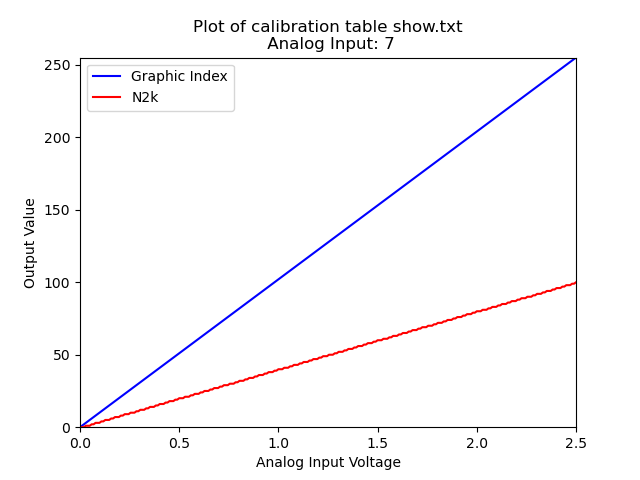
\includegraphics[width=\linewidth]{show.txt.png}
  \centering
  \caption{Sample Visualizationl}
  \label{fig:Sample}
\end{figure}

%Figure \ref{fig:Sample} shows a sample Calibration Table Visualization

The x-axis represents the voltage at the input of the Analog to Digital block. The first row of the table is accessed at the left, corresponding to 0.0 volts and the last table is at the far right at 2.5 volts.  The vertical axis values are pulled from the corresponding row in the Calibration Table.. For example, the last row of this Calibration  Table contains a Graphic index of 255 and NMEA 2000 value of 100.
  
The next step is to show several examples of increasing complexity to illustrate the power of the Calibration Tables to accommodate a wide variety of sensors.

\section{Example 1}
This example implements a gauge that displays the distance to the dock, given a sensor that  senses distance and has a linear scale of 0 - 2.5 V, representing 0 - 25 feet.   NMEA 2000 data will not be used with this example, so it is set to 0.  With the sensor voltage swing of 0 to 2.5 V, no input conditioning is needed. A dial type gauge will be used, designed so the pointer reads higher with decreasing distance. So, the scale starts out at 25 feet and decreases to 0 feet at full scale.
At 0 feet, the vDash style gauge will be full scale, decreasing as the sensor starts supplying voltage

\begin{figure}[hbt!]
  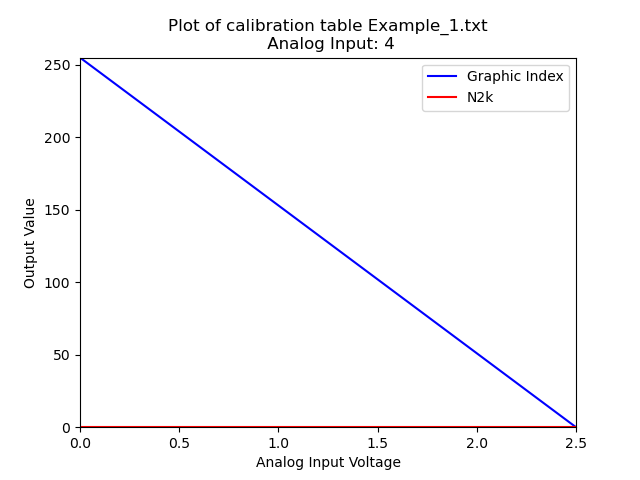
\includegraphics[width=\linewidth]{Example_1.txt.png}
  \centering
  \caption{Example 1 visualization}
  \label{fig:Example_1}
\end{figure}

%Figure \ref{fig:Example_1} shows the Example 1 visualization

\section{Example 2}
Same problem as Example 1, but the original sensor has broken and all the Sensor Store has is a unit that still outputs 0 - 2.5 V, but has a range of 50 feet.  The captain is used to the gauge reading 25 to 0 feet and doesn’t want to change.  The Calibration Table needs to be modified so it scales when the sensor detects 25 feet, which is now at 1.25 volts.  The resulting table looks like this

\begin{figure}[hbt!]
  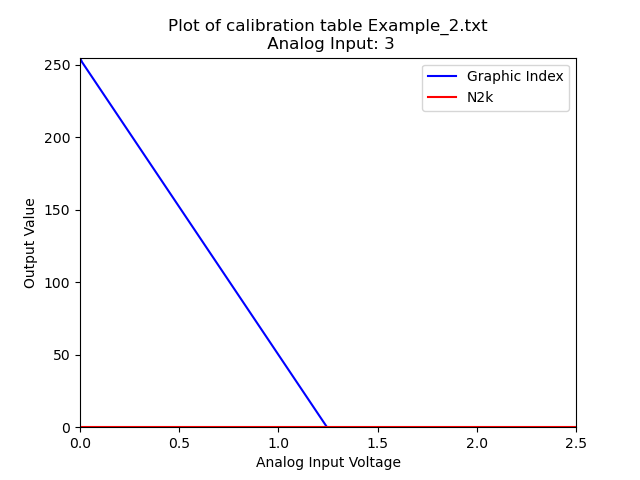
\includegraphics[width=\linewidth]{Example_2.txt.png}
  \centering
  \caption{Example 2 visualization}
  \label{fig:Example_2}
\end{figure}

%Figure \ref{fig:Example_2} shows the Example 2 visualization

As the sensor continues to output increasing voltage between 25 to 50 feet, the Graphic Index remains at 0.

\section{Example 3}
Yet another sensor breaks, and now the Sensor Store has 25 foot sensors in stock, but instead of 0 - 2.5 V, this new sensor outputs  0.5  -  2.5 V for 0 - 25 feet.  This may be useful in situations where it may be useful to determine if the sensor is actually reading 0 feet, or disconnected. The Calibration Table Graphic Index output has to be full scale starting at 0.5 V, (representing 0 feet) and scale down to 25 feet at 2.5 V.  We could take advantage of the Display Value to display ‘Dead’ or something similar for the first couple of Calibration Table rows to detect the disconnected case. 

\begin{figure}[hbt!]
  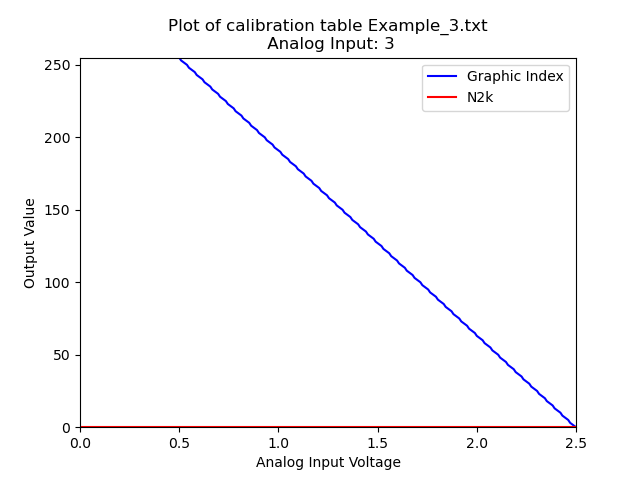
\includegraphics[width=\linewidth]{Example_3.txt.png}
  \centering
  \caption{Example 3 visualization}
  \label{fig:Example_3}
\end{figure}

\section{Example 4}
 NMEA 2000 data has its own set of scaling.  Examining PGN 127489 Engine Parameters Dynamic;  field Oil Pressure, the G2 user’s manual shows a range of 0 - 237 psi.  For this example,  after conditioning, the oil pressure sensor voltage has a range of 0.0 - 2.0 volts, corresponding to 0 - 120 psi.  The vDash style gauge will be configured for the same range, 0 - 120 psi. The NMEA 2000 scaling works the same way.  120 psi represents 51\% of the NMEA 2000 range of 0 - 237 psi.  The NMEA 2000 output value must therefore be 51\% of 255 at 120 psi or row index 130.  With linear scaling, that is all the information needed to establish the NMEA 2000 curve.
\begin{figure}[hbt!]
  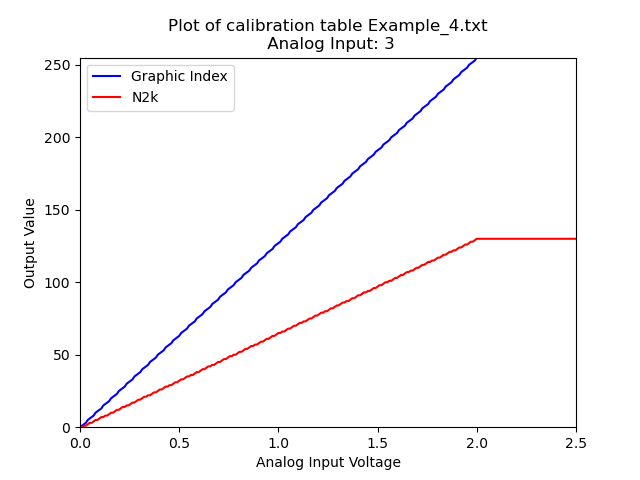
\includegraphics[width=\linewidth]{Example_4.txt.png}
  \centering
  \caption{Example 4 visualization}
  \label{fig:Example_4}
\end{figure}

\section{Example 5}
 This example brings it all together to use a commercial sensor to implement an engine temperature gauge.  The NMEA 2000 PGN that will be used is 127489 Engine Dynamic Parameters; field Engine Temperature.  The vDash gauge will be configured from 100 to 260F. The sensor in this example is a common VDO 250F.  It is a resistance that drops as the temperature rises.  The sender curve looks like this;
\begin{figure}[hbt!]
  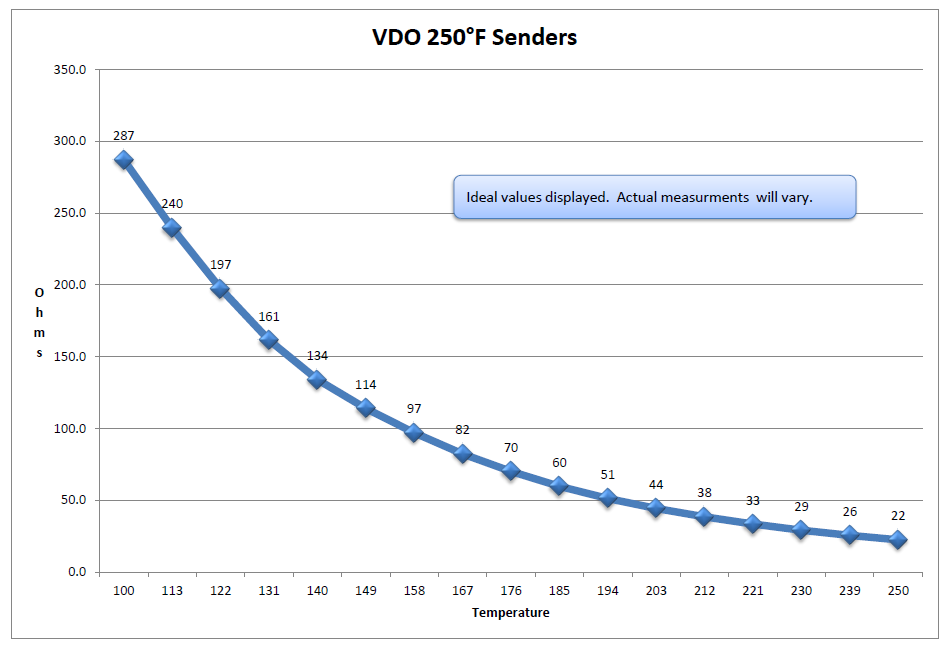
\includegraphics[width=\linewidth]{VDO sensor curve.png}
  \centering
  \caption{VDO Sender curve}
  \label{fig:Sender Curve}
\end{figure}

Recall that we need sensors to supply voltage to the Analog to Digital block.  One of the Input Conditioning options provides a 300 Ohm pullup resistor to 2.5V for some of the Analog Inputs. When configured this way, the voltage presented to the Analog to Digital block is equal to$ (Sensor\_resistance  * 2.5 ) / (Sensor\_resistance + 300)$.  For example, a temperature  of 185 F corresponds to 60 ohms.  This would yield a voltage of $(60 * 2.5) / (60 + 300)$ or 0.42V.  To calculate the Calibration Table row index that corresponds to 185F ,
 use $ Sensor\_voltage * 256 / 2.5 $  or table row index 43. 
Next, we need to determine what data to place in this table row.  
\begin{itemize}
\item NMEA 2000 data
The G2 has predefined the range for the 127489 PGN; field Engine Temperature as -20 - 278F. To convert the 185F temperature to an NMEA 2000 output value, use $ (Temperature + 20) * (278 -  (-20))/255 $.  For 185F, this would be 175
\item Graphic Index value
The gauge is defined as 100 - 260F.  For the Graphic Index, calculate $(Temperature - 100) / (260 - 100) * 255$  In this case, 135 
\end{itemize}

This completes the data needed for row 43.  The rest of the points can be generated in a similar fashion.  Intermediate points are usually linear, as if you drew a line between the two defined points and filled in the values.  When this process is complete, the resulting data looks much


\begin{figure}[hbt!]
  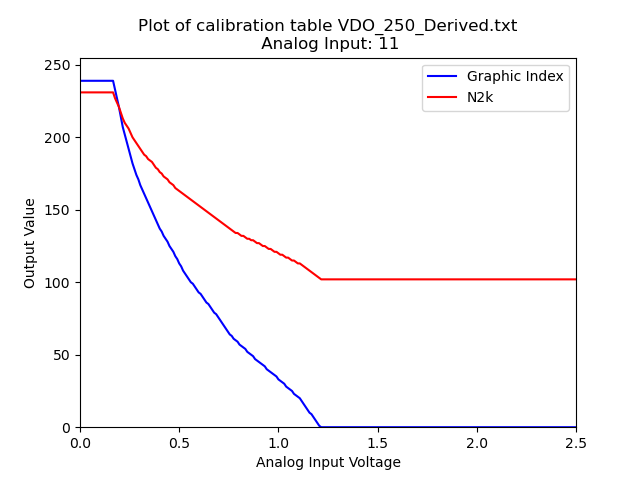
\includegraphics[width=\linewidth]{VDO_250_Derived.txt.png}
  \centering
  \caption{Example 5 visualization}
  \label{fig:Example_5}
\end{figure}

\section{NMEA 2000 ranges}
The easiest way to think of an NMEA 2000 range is if there had been a vDash style gauge configured to the same range and the goal was to figure out the correct Graphic Index curve to display the correct values.  The G2 unit handles whatever scaling and offsets required to build and emit the required PGNs  Using the previous example, if we had defined the vDash style gauge to be -20 - 278F, the Graphic Index values would be identical to the NMEA 2000 values

\subsection{A word about NMEA 2000 scaling}
While not required to build correct Calibration Tables, it may be useful to understand the internals of NMEA 2000 scaling.  In general, this scaling may be different for every NMEA field

To give an idea about what happens in the NMEA 2000 scaling block, consider PGN 127489 - Engine Parameters Dynamic: Fuel  Pressure.  The G2 User’s Manual gives the range as 0 - 74 psi. That means each output unit from the Calibration Table is $ (74 / 256 )$ or 0.29 psi.  In the 127489 PGN record, the Fuel Pressure field is stored in units of kPa.  1 psi is 6.895 kPa.  So, each Calibration Table unit is  $(6.895 * 0.29 )$ or 2.0 kPa.   The NMEA 2000 scaling block for this field multiplies the Calibration Table output by 2 before storing into the PGN field.  This all happens automatically; and produces the correct values as long as the proper range values are used for the NMEA 2000 table entries.

\section{Input Conditioning}\label{Input Conditioning}
There are three types of input conditioning built into the G2, two of which are fixed and one configurable with switches on the G2 unit.  Each Analog input has one type of input conditioning.  Analog Inputs 8 \& 11 have  Type A.  Analog Inputs 5 \& 6, Type B.  The remainder (0 -4, 7, 9-10) Type C. Note that the following descriptions are for the default configuration


\subsection{Type A Input}
Type A inputs provide a voltage scaling function.  Analog inputs support the range 0 - 2.5 v.  The voltage divider equation is $ R_{series} / (R_{series} + R_{pulldown})$  or $100K / (100K + 10K)$ =  1/11 or 0.09.  This means that a sensor connected to this type of input will be scaled by a factor of 11. Another way to look at it is the valid  input voltage range is 0 - 27.5 V

\begin{figure}[hbt!]
  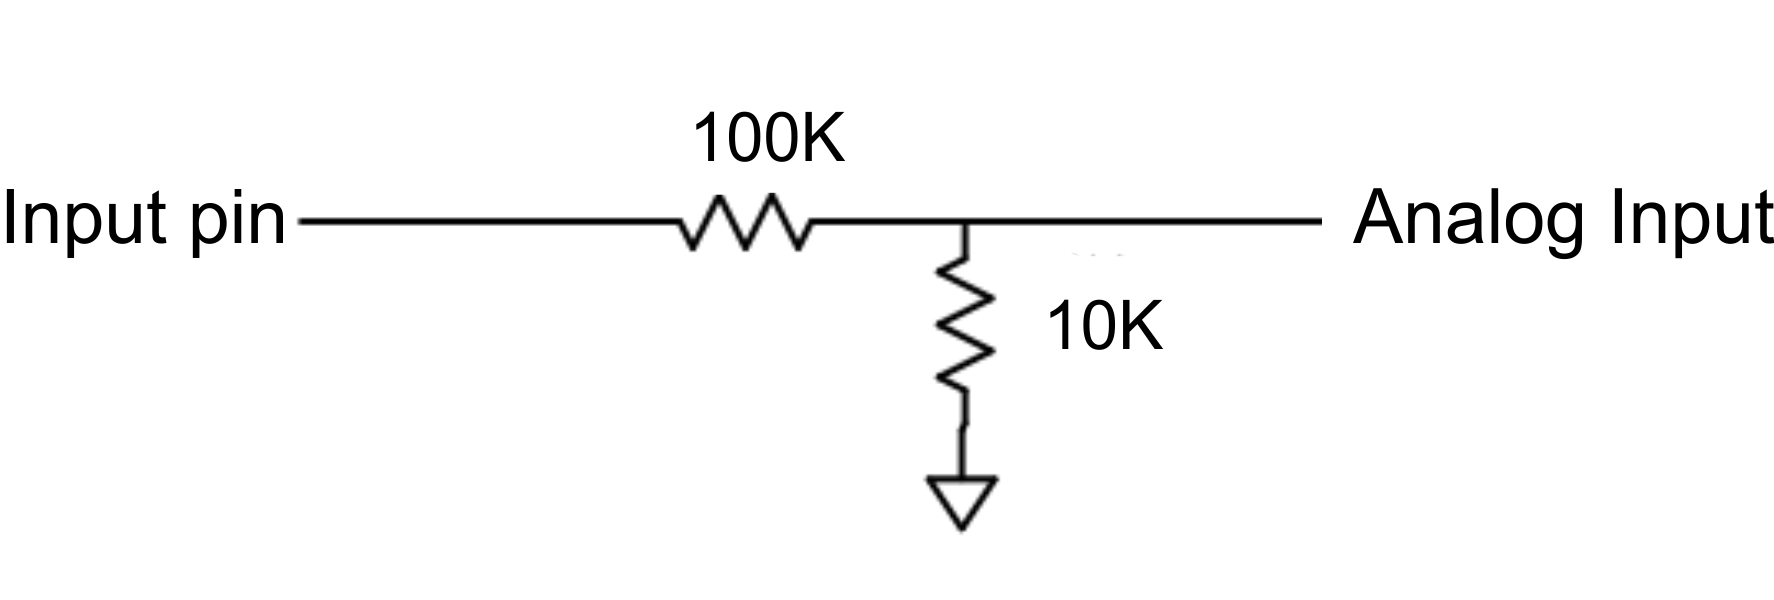
\includegraphics[scale=0.7]{Type A input.png}
  \centering
  \caption{Type A Input}
  \label{fig:Type A}
\end{figure}



\subsection{Type B Input}
\begin{figure}[hbt!]
  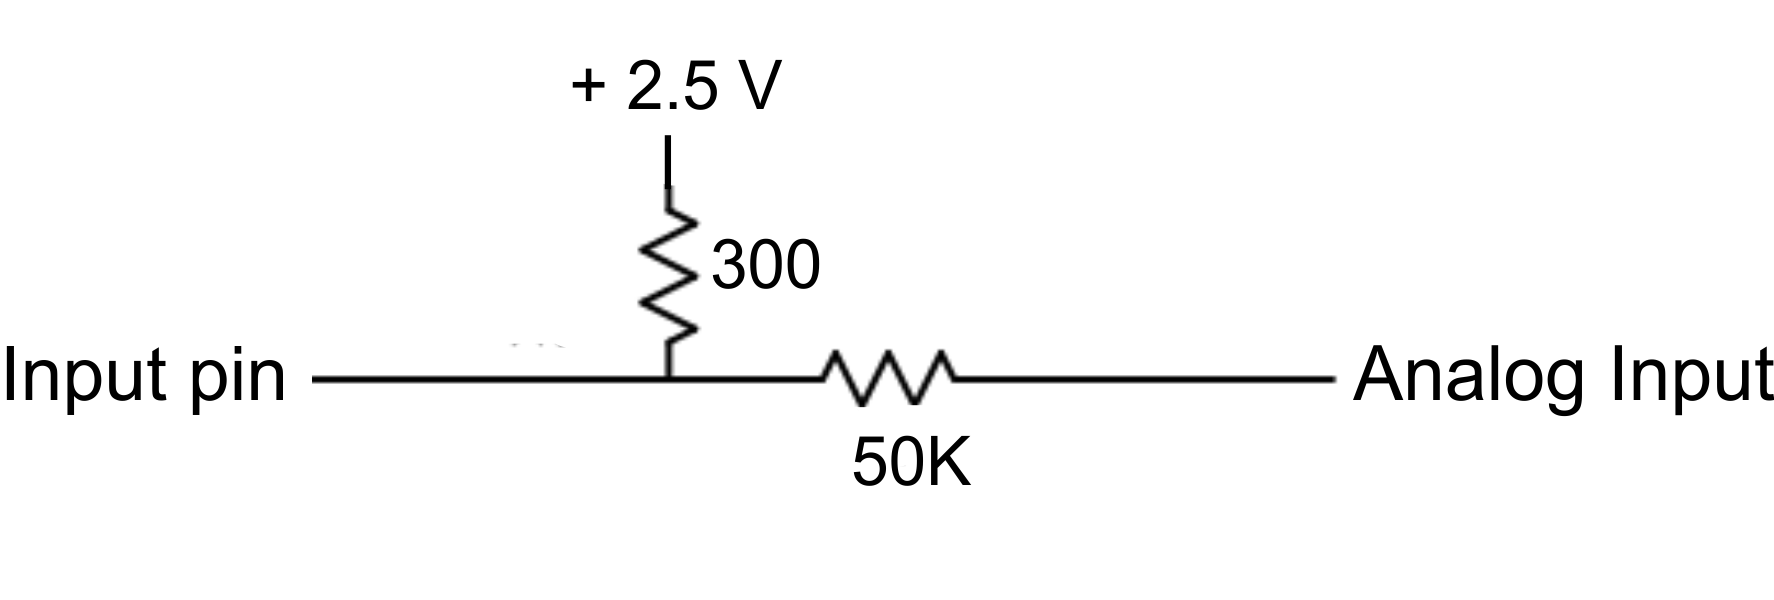
\includegraphics[scale=0.7]{Type B input.png}
  \centering
  \caption{Type B Input}
  \label{fig:Type B}
\end{figure}

Type B inputs can be used for sensors that operate by resistance and have no ability to provide voltage on their own.  A good example are VDO type temperature senders, whose resistance varies in the 30 - 300 ohm range.  When used in this configuration, analog input voltage is calculated as $ (2.5 * Sensor\_resistance)/(Sensor\_resistance + 300)$.  For the resistance range here, the Analog Input voltage would range from 0.22 - 1.25 V. (Example 5 uses a sensor of this type)

\subsection{Type C Input}
Because of its configurability, a Type C input is the most versatile.  Not all switch combinations are useful.  Consult the table for details. 
\begin{figure}[hbt!]
  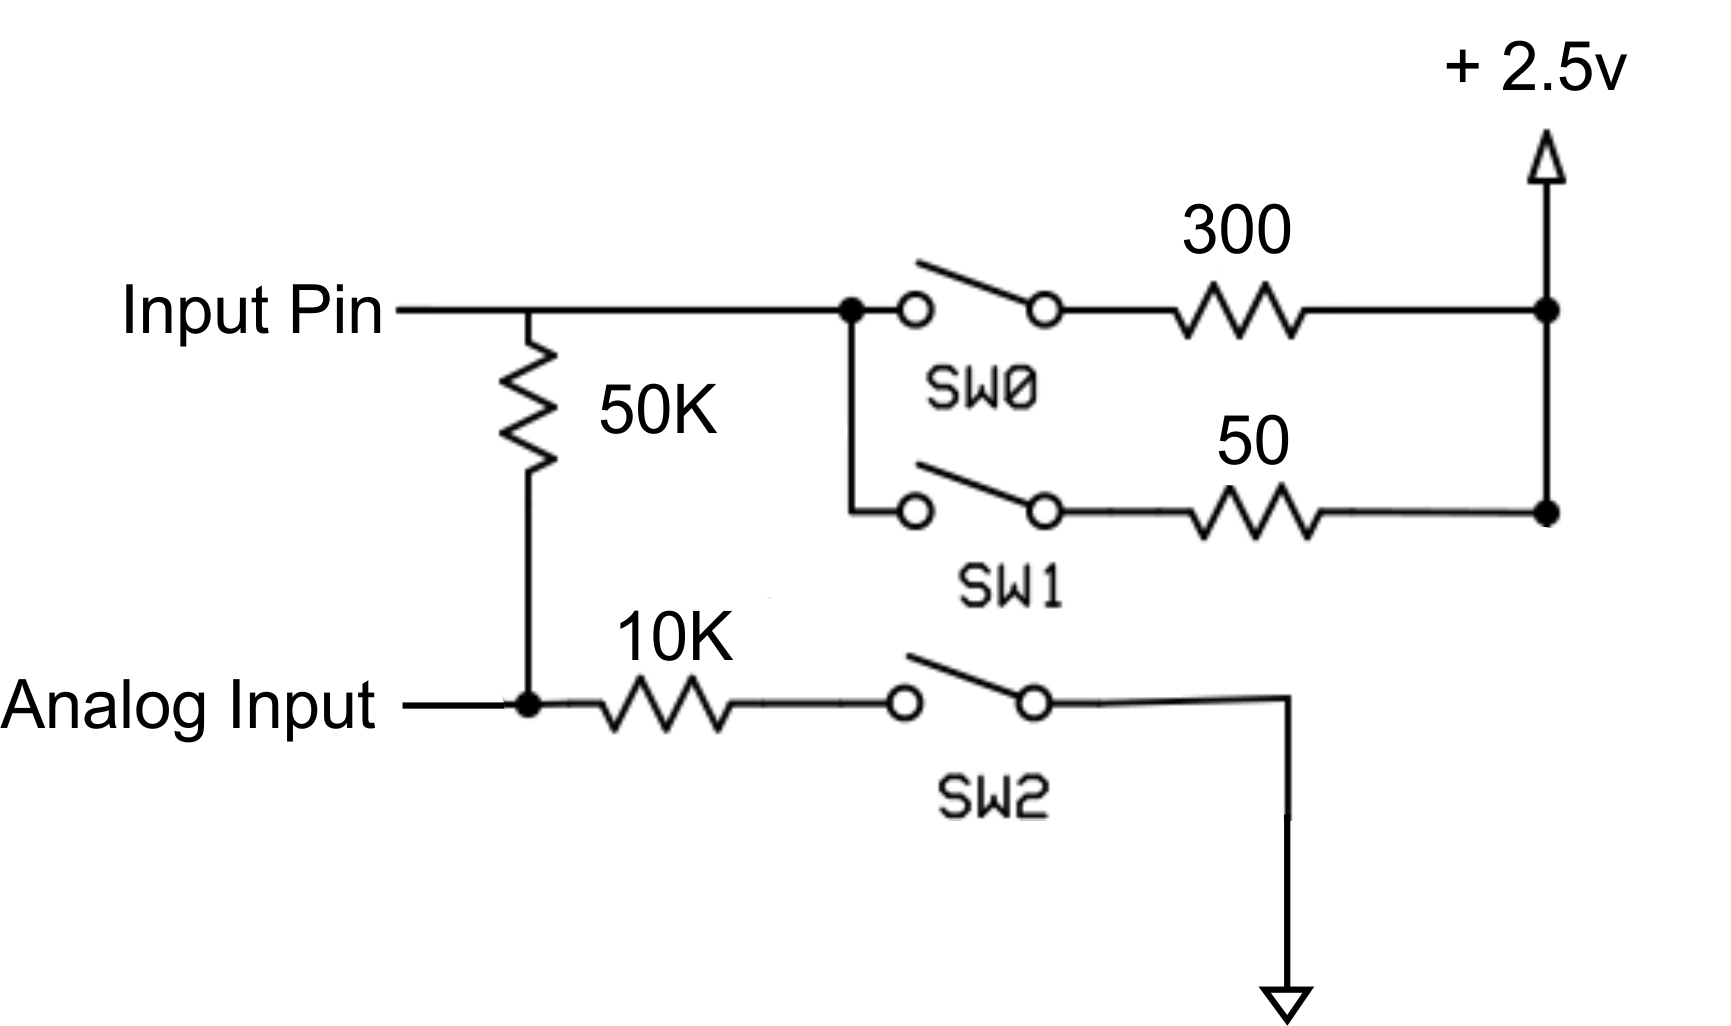
\includegraphics[scale=0.7]{Type C input.png}
  \centering
  \caption{Type C Input}
  \label{fig:Type C}
\end{figure}

\begin{figure}[hbt!]
  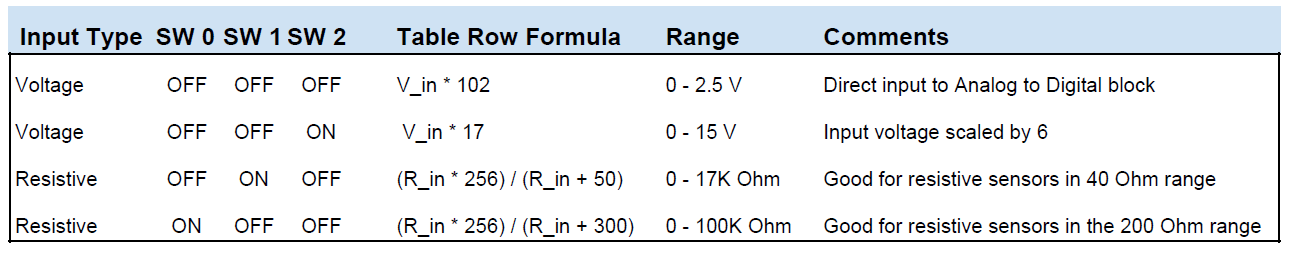
\includegraphics[width=\linewidth]{Switch Settings.png}
  \centering
  \caption{Type C Input Switch Table}
  \label{fig:Type C Switch Table}
\end{figure}

\section{Conclusions}
In this application note, the following items have been discussed

\begin{itemize}
\item Purpose and format of a Calibration Table \cite[Calibration Tables]{G2}
\item Description of an Analog Input Channel
\item G2 Input Conditioning configurations
\item Graphic Index and NMEA 2000 consideration
\end{itemize}

\begin{thebibliography}{9}
\bibitem[G2]{G2} Chetco G2 User's Manual
\end{thebibliography}
 
\end{document}